%%%%%%%%%%%%%%%%%%%%%%%%%%%%%%%%%%%%%%%%%
% Structured General Purpose Assignment
% LaTeX Template
%
% This template has been downloaded from:
% http://www.latextemplates.com
%
% Original author:
%  Ted Pavlic (http://www.tedpavlic.com)
% Modified by:
%  Joe Del Rocco (https://joe.delrocco.org)
%%%%%%%%%%%%%%%%%%%%%%%%%%%%%%%%%%%%%%%%%

%----------------------------------------------------------------------------------------
%  PACKAGES AND CONFIGURATION
%----------------------------------------------------------------------------------------

\documentclass[fleqn]{article}
\usepackage{geometry}
\usepackage{fancyhdr} % For custom headers
\usepackage{lastpage} % To determine the last page for the footer
\usepackage{extramarks} % For headers and footers
\usepackage[most]{tcolorbox} % For problem answer sections
\usepackage{graphicx} % For inserting images
\usepackage{xcolor} % For link coloring
\usepackage[hidelinks]{hyperref} % For URL links (no box or color name)
\usepackage{bm}
\usepackage{amsmath}
\usepackage{amssymb}
\usepackage[english]{babel}
\usepackage[utf8x]{inputenc}
\usepackage{amsmath}
\usepackage{tikz}
\usetikzlibrary{arrows,automata}

% Margins
\geometry{
a4paper,
tmargin=1in,
bmargin=1in,
lmargin=1in,
rmargin=1in,
textwidth=6.5in,
textheight=9.0in,
headsep=0.25in
}

% Header and footer
\pagestyle{fancy}
\lhead{\myName} % Top left header
\chead{\myCourse: \myAssignment} % Top center header
\rhead{\firstxmark} % Top right header
\lfoot{\lastxmark} % Bottom left footer
\cfoot{} % Bottom center footer
\rfoot{Page\ \thepage\ of\ \pageref{LastPage}} % Bottom right footer
\renewcommand\headrulewidth{0.4pt} % Size of the header rule
\renewcommand\footrulewidth{0.4pt} % Size of the footer rule

% Other configurations
\setlength\parindent{0pt} % Removes all indentation from paragraphs
\setlength\parskip{1pt} % Ensures paragraphs are still recognizable as such
\setcounter{secnumdepth}{0} % Removes default section numbers
\setcounter{tocdepth}{3} % Sets depth of table of contents
\linespread{1.1}

% Template values
% \newcommand{\myLogo}{starfleet.jpg}
\newcommand{\myName}{Manish Yadav}
\newcommand{\myJobTitle}{3836-6483}
\newcommand{\myCompany}{Starfleet Academy}
\newcommand{\myLocation}{1701 Lincoln Blvd, San Francisco, CA}
\newcommand{\myURL}{www.starfleet.edu}
\newcommand{\myEmail}{m.yadav@ufl.edu}
\newcommand{\myCourse}{CNT5106C}
\newcommand{\mySection}{Fall 2020}
\newcommand{\myTeacher}{Dr. Ye Xia}
\newcommand{\myAssignment}{Homework 3}
\newcommand{\myDueDate}{Fri,\ Oct\ 9,\ 2020}
\newcommand{\norm}[1]{\left\lVert#1\right\rVert}


%----------------------------------------------------------------------------------------
%  DOCUMENT STRUCTURE (MACROS & ENVIRONMENTS)
%----------------------------------------------------------------------------------------

% Colored links macro
\newcommand{\hrefcol}[3] {\href{#1}{\textcolor{#3}{#2}}}

% Creates a counter to keep track of the number of problems
\newcounter{homeworkProblemCounter}

% Macro for custom title page signature header
\newsavebox{\myTitleSignature}
\sbox{\myTitleSignature}{%
\begin{tabular*}{\textwidth}{@{}l@{}@{\extracolsep{0.125in}}l@{}}%
\parbox[c][]{2.5in}{{\textbf{\myName} \par}
                    {\small \myJobTitle \par}
                    {\small \hrefcol{mailto:\myEmail}{\myEmail}{blue}} \par}
\end{tabular*}}

% Header and footer for when a page split occurs within a problem environment
\newcommand{\enterProblemHeader}[1]{%
\nobreak\extramarks{#1}{#1 continued on next page\ldots}\nobreak%
\nobreak\extramarks{#1 (continued)}{#1 continued on next page\ldots}\nobreak%
}

% Header and footer for when a page split occurs between problem environments
\newcommand{\exitProblemHeader}[1]{%
\nobreak\extramarks{#1 (continued)}{#1 continued on next page\ldots}\nobreak%
\nobreak\extramarks{#1}{}\nobreak%
}

\newcommand{\homeworkProblemName}{} % Argument = name of problem; default = "Problem #"
\newenvironment{homeworkProblem}[1][Problem \arabic{homeworkProblemCounter}]{%
\stepcounter{homeworkProblemCounter}% % Increase counter for number of problems
\renewcommand{\homeworkProblemName}{#1}% % Assign \homeworkProblemName the argument
\section{\homeworkProblemName}% % Make a section in the document with the custom problem count
\enterProblemHeader{\homeworkProblemName}% % Header and footer within environment
}{%
\exitProblemHeader{\homeworkProblemName}% % Header and footer after environment
}

\newcommand{\problemAnswer}[1]{ % Defines the problem answer command with the content as the only argument
\begin{tcolorbox}[breakable,enhanced,colback=gray!5!white,title=Answer]%
#1
\end{tcolorbox}%
% Alternative - Makes the box around the problem answer and puts the content inside
%\noindent\framebox[\columnwidth][c]{\begin{minipage}{0.98\columnwidth}#1\end{minipage}}
}

\newcommand{\homeworkSectionName}{}
\newenvironment{homeworkSection}[1]{% % For sections w/in problems; Argument = name of section (no default)
\renewcommand{\homeworkSectionName}{#1}% % Assign \homeworkSectionName the argument
\subsection{\homeworkSectionName}% % Make a subsection with the name of the subsection
\enterProblemHeader{\homeworkProblemName\ [\homeworkSectionName]}% % Header and footer within environment
}{%
\enterProblemHeader{\homeworkProblemName}% % Header and footer after environment
}

%----------------------------------------------------------------------------------------
%   TITLE PAGE
%----------------------------------------------------------------------------------------
\begin{document}

% Blank out the traditional title page
\title{\vspace{-1in}} % no title name
\author{} % no author name
\date{} % no date listed
\maketitle % makes this a title page

% Use custom title macro instead
\usebox{\myTitleSignature}
\vspace{1in} % spacing below title header

% Assignment title
{\centering \huge \myAssignment \par}
{\centering \noindent\rule{4in}{0.1pt} \par}
\vspace{0.05in}
{\centering \myCourse~: \mySection~: \myTeacher \par}
{\centering Due \myDueDate \par}
%{\centering Prepared w/ \LaTeX \par}
\vspace{1in}

% Table of Contents
\tableofcontents
\newpage

%----------------------------------------------------------------------------------------
%	PROBLEM 1
%----------------------------------------------------------------------------------------

%\begin{homeworkProblem}[Exercise \#\arabic{homeworkProblemCounter}] % Use for custom section title
\begin{homeworkProblem}
\begin{homeworkSection}{P5}
Suppose that the UDP receiver computes the Internet checksum for the received UDP segment and finds that it matches the value carried in the checksum field. Can the receiver be absolutely certain that no bit errors have occurred? Explain. \\
\problemAnswer{
    No. The receiver cannot be certain that no bit errors have occurred. \\
    
    It may be possible that both data and checksum have been corrupted that could result in checksum matched at the receiving end \cite{stone2000crc}. \\
    
    Also, 2-bit error changes in different word (i.e $1 \rightarrow 0$ and $0 \rightarrow 1$) will not change the sum. Because checksum is merely an addition. Consider two bytes (trimmed down example of WORD) $0000 0101$ and $0000 0011$, this would result in a sum of $0000 1000$. But if 1 bit from each of the bytes is flipped, i.e $0000 0111$ and $0000 0001$ would result in a sum of $0000 1000$ which is the same. \\
    
    It could also fail to detect if there is a transposition of the word i.e. $0011$ and $0101$ is being transmitted instead of $0101$ and $0011$
    
}
\end{homeworkSection}
\end{homeworkProblem}
%----------------------------------------------------------------------------------------
\pagebreak

\begin{homeworkProblem}
\begin{homeworkSection}{P6}
Consider our motivation for correcting protocol \texttt{rdt2.1}. Show that the receiver, shown in \textbf{Figure 3.57}, when operating with the sender shown in \textbf{Figure 3.11}, can lead the sender and receiver to enter into a deadlock state, where each is waiting for an event that will never occur \\
\problemAnswer{
    The real problem lies with the fact that the sender has to receive an acknowledgment from the receiver in order to send the next packet. \\
    
    To best illustrate this scenario, consider a scenario where the receiver received a packet, sent an ACK, and now has moved to wait for another packet 0. However, the ACK sent is corrupted and the sender sends back packet 1 again. Now, both the sender and receiver have entered a state where they keep sending packet 1 and the receiver keeps sending NACK since it is now waiting for packet 0 to arrive.
}
\end{homeworkSection}
\end{homeworkProblem}
%----------------------------------------------------------------------------------------
\pagebreak

\begin{homeworkProblem}
\begin{homeworkSection}{P12}
The sender side of \texttt{rdt3.0} simply ignores (that is, takes no action on) all received packets that are either in error or have the wrong value in the \texttt{acknum} field of an acknowledgment packet. Suppose that in such circumstances, \texttt{rdt3.0} were simply to retransmit the current data packet. Would the protocol still work? (Hint: Consider what would happen if there were only bit errors; there are no packet losses but premature timeouts can occur. Consider how many times the $n^{th}$ packet is sent, in the limit as $n$ approaches infinity.) \\
\problemAnswer{
    Yes. The protocol would still work. There would be packet re-transmission in case if the ACK was completely lost or had errors.\\
    
    Consider a case where packet 1 was sent. In case of premature timeout, an extra copy would be sent that would be ACK'd by the receiver. This would cause the sender to send an extra copy of packet 2. This extra copy would be ACK'd along with the previous one causing packet 3 to be sent twice. This process continues to repeat on and on. Since $n$ approaches infinity, the number of the packet sent would tend towards infinity as well.
}
\end{homeworkSection}
\end{homeworkProblem}
%----------------------------------------------------------------------------------------
\pagebreak

\begin{homeworkProblem}
\begin{homeworkSection}{P13}
Consider the \texttt{rdt 3.0} protocol. Draw a diagram showing that if the network connection between the sender and receiver can reorder messages (that is, that two messages propagating in the medium between the sender and receiver can be reordered), then the alternating-bit protocol will not work correctly (make sure you clearly identify the sense in which it will not work correctly). Your diagram should have the sender on the left and the receiver on the right, with the time axis running down the page, showing data (D), and acknowledgment (A) message exchange. Make sure you indicate the sequence number associated with any data or acknowledgment segment. \\
\problemAnswer{
    \begin{center}
        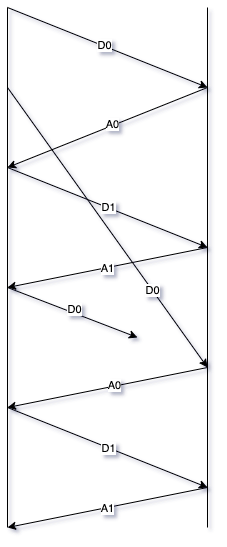
\includegraphics[width=0.25\columnwidth]{13.png}
    \end{center}
    \texttt{rdt 3.0} works correctly under the assumption of a FIFO based channel. In case of packet reordering, it causes \texttt{rdt 3.0} to deliver incorrect data. As in the above case, the older of D0 gets accepted.
}
\end{homeworkSection}
\end{homeworkProblem}
%----------------------------------------------------------------------------------------
\pagebreak

\begin{homeworkProblem}
\begin{homeworkSection}{P15}
Consider the cross-country example shown in \textbf{Figure 3.17} . How big would the window size have to be for the channel utilization to be greater than 98 percent? Suppose that the size of a packet is 1,500 bytes, including both header fields and data. \\
\problemAnswer{
    \begin{equation*}
        d_{trans} = \frac{L}{R} = \frac{1500 * 8}{10^9} = 0.012ms
    \end{equation*}
    In order to get channel utilization,
    \begin{align*}
        U &=  N * \frac{L/R}{RTT + L/R} = \frac{N * 0.012}{30 + 0.012} \\
        \frac{98}{100} & =  \frac{N * 0.012}{30.012} \\
        N &= 2451
    \end{align*}
    \textbf{Therefore the window size should be at least 2451.}
}
\end{homeworkSection}
\end{homeworkProblem}
%----------------------------------------------------------------------------------------
\pagebreak

\begin{homeworkProblem}
\begin{homeworkSection}{P19}
Consider a scenario in which Host A wants to simultaneously send packets to Hosts B and C. A is connected to B and C via a broadcast channel—a packet sent by A is carried by the channel to both B and C. Suppose that the broadcast channel connecting A, B, and C can independently lose and corrupt packets (and so, for example, a packet sent from A might be correctly received by B, but not by C). Design a stop-and-wait-like error-control protocol for reliably transferring packets from A to B and C, such that A will not get new data from the upper layer until it knows that both B and C have correctly received the current packet. Give FSM descriptions of A and C. (Hint: The FSM for B should be essentially the same as for C.) Also, give a description of the packet format(s) used. \\
\problemAnswer{
The below diagrams illustrates three host A, B and C. The first diagrams illustrates the sender state indicating where the channel may lose message on B/C or both. In order to make sure the receiver has received message we make use of sequence number that ensures that receiver does not get the same message again. Hence with sequence number, the sender mechanism should be able to work. \\
    \textbf{Sender}
    \begin{center}
        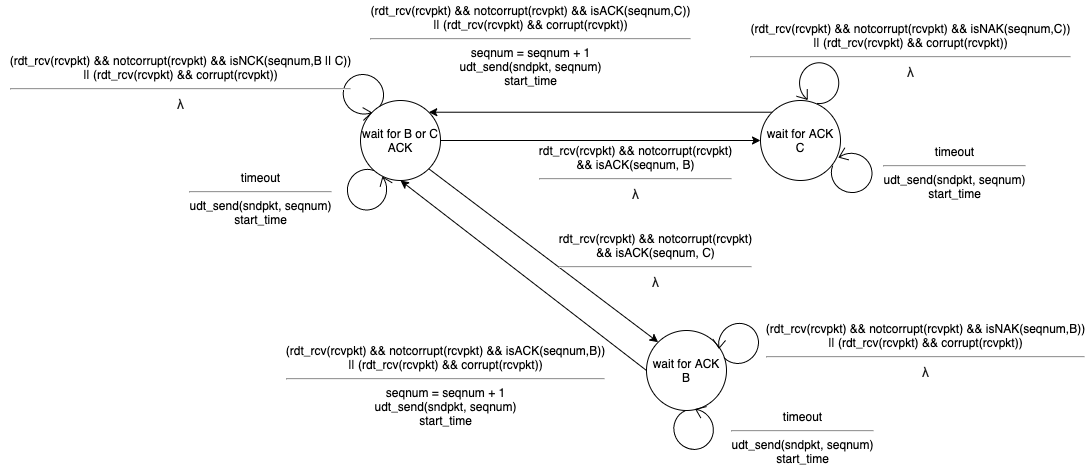
\includegraphics[width=1.0\columnwidth]{19.png}
    \end{center}
    \textbf{Receiver}
    \begin{center}
        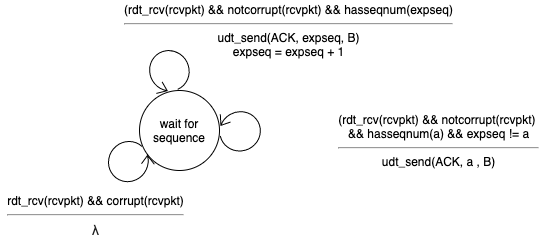
\includegraphics[width=0.75\columnwidth]{19_receiver.png}
    \end{center}

}
\end{homeworkSection}
\end{homeworkProblem}
%----------------------------------------------------------------------------------------
\pagebreak


\begin{homeworkProblem}
Consider the GBN protocol with a sender window size of 4 and a sequence number range of 1,024. Suppose that at time t, the next in-order packet that the receiver is expecting has a
sequence number of k. Assume that the medium does not reorder messages. Answer the following questions:
\begin{homeworkSection}{P22 a}
What are the possible sets of sequence numbers inside the sender’s window at time t? Justify your answer. \\
\problemAnswer{
    At the time $t$, the receiver would get packet $k$, meaning packets from $[k - 4...k - 1]$ has been received already. If all of these packets are ACK'd then the window is $[k, k + 3]$. Also packet $k$ to packet $k + 3$ maybe already sent from sender side. 

    Therefore sender's window is $[k - 4, k]$. In case the beginning of the window is at $k$, then packet sequence will be from $[k, k + 3]$
}
\end{homeworkSection}

\begin{homeworkSection}{P22 b}
What are all possible values of the ACK field in all possible messages currently propagating back to the sender at time t? Justify your answer. \\
\problemAnswer{
    Same as above, $\text{ACK }{k - 5}$ to $\text{ACK }{k - 1}$ has already sent from receiver. Additionally, the receiver may be just received packet $k - 1$ at time $t$, in this case, the previous ACKs are still propagating. 
}
\end{homeworkSection}
\end{homeworkProblem}
%----------------------------------------------------------------------------------------
\pagebreak


\begin{homeworkProblem}
\begin{homeworkSection}{P23}
Consider the GBN and SR protocols. Suppose the sequence number space is of size k. What is the largest allowable sender window that will avoid the occurrence of problems such as that in Figure 3.27 for each of these protocols? \\
\problemAnswer{
    The largest allowable sender window that will avoid the occurrence of the problem in Figure 3.27 would have to be less than or equal to half of the sequence number space size \cite{kurose2010computer}.
}
\end{homeworkSection}
\end{homeworkProblem}
%----------------------------------------------------------------------------------------
\pagebreak

\begin{homeworkProblem}
Answer true or false to the following questions and briefly justify your answer:

\begin{homeworkSection}{P24 a}
With the SR protocol, it is possible for the sender to receive an ACK for a packet that falls outside of its current window \\
\problemAnswer{
		True. This is possible in case the receiver's ACKs are received after the sender is timed out. As the second group of ACKs for the would-be resent even if the window has advanced past those packets.

}
\end{homeworkSection}

\begin{homeworkSection}{P24 b}
With GBN, it is possible for the sender to receive an ACK for a packet that falls outside of its current window. \\
\problemAnswer{
    True. Same as P24 a.
}
\end{homeworkSection}

\begin{homeworkSection}{P24 c}
The alternating-bit protocol is the same as the SR protocol with a sender and receiver window size of 1. \\
\problemAnswer{
    True.
}
\end{homeworkSection}

\begin{homeworkSection}{P24 d}
The alternating-bit protocol is the same as the GBN protocol with a sender and receiver window size of 1. \\
\problemAnswer{
    True. A window size of 1 avoids the packet from being out of order.
}
\end{homeworkSection}
\end{homeworkProblem}
%----------------------------------------------------------------------------------------
\pagebreak

\begin{homeworkProblem}
Host A and B are communicating over a TCP connection, and Host B has already received from A all bytes up through byte 126. Suppose Host A then sends two segments to Host B back-to-back. The first and second segments contain 80 and 40 bytes of data, respectively. In the first segment, the sequence number is 127, the source port number is 302, and the destination port number is 80. Host B sends an acknowledgment whenever it receives a segment from Host A.
\begin{homeworkSection}{P27 a}
In the second segment sent from Host A to B, what are the sequence number, source port number, and destination port number? \\
\problemAnswer{
    Sequence number = 127+80 = 207\\ Source port number = 302 \\ Destination port number
= 80
}
\end{homeworkSection}

\begin{homeworkSection}{P27 b}
If the first segment arrives before the second segment, in the acknowledgment of the first arriving segment, what is the acknowledgment number, the source port number, and the
destination port number?\\
\problemAnswer{
    Acknowledgment number = 207\\
Source port number = 80 \\
Destination port number = 302
}
\end{homeworkSection}
\begin{homeworkSection}{P27 c}
If the second segment arrives before the first segment, in the acknowledgment of the first arriving segment, what is the acknowledgment number? \\
\problemAnswer{
    In the event of the second segment arriving before the first segment, the acknowledgment number would be 127 since it is missing a segment of 80 bytes which has to be delivered to maintain the order.
}
\end{homeworkSection}
\begin{homeworkSection}{P27 d}
Suppose the two segments sent by A arrive in order at B. The first acknowledgment is lost and the second acknowledgment arrives after the first timeout interval. Draw a timing diagram, showing these segments and all other segments and acknowledgments sent. (Assume there is no additional packet loss.) For each segment in your figure, provide the sequence number and the number of bytes of data; for each acknowledgment that you add, provide the acknowledgment number. \\
\problemAnswer{
    \begin{center}
        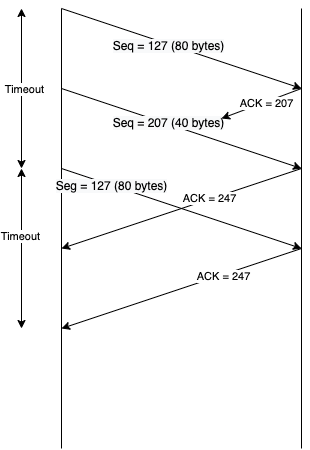
\includegraphics[width=0.25\columnwidth]{22.png}
    \end{center}
    Left side = Host A, Right side = Host B
}
\end{homeworkSection}

\end{homeworkProblem}
\pagebreak
\bibliographystyle{plain}
\bibliography{references} % see references.bib for bibliography management
\end{document}
%----------------------------------------------------------------------------------------
%	DONE
%----------------------------------------------------------------------------------------
